\documentclass[10pt,a4paper]{article}
\usepackage{amsmath,amssymb,amsthm,graphicx}
\usepackage{amsmath,amssymb,amsthm,mathtools,graphicx,enumitem}
\usepackage[no-math]{fontspec}
\newenvironment{authorclaim}[1]{\par\medskip\noindent\textbf{#1.}\ \ignorespaces}{\par\medskip}
\DeclareMathOperator{\PSP}{PSP}
\allowdisplaybreaks
\title{Super-quadratic wire lower bound for general depth-four arithmetic circuits over characteristic zero}
\author{Nikhil Gupta, Chandan Saha, Bhargav Thankey}
\date{doi:10.4230/LIPIcs.CCC.2020.23; CC BY 3.0 Unported}
\begin{document}
\maketitle
\noindent\textit{Editorial scope.} Single complete characteristic-zero depth-four lower-bound mechanism with all pruning and parameter support; no independent mathematical repair or proof certification.\par\medskip
\noindent\textit{Allowed standard prerequisites (editorial).}\begin{itemize}
\item Arithmetic circuits, VNP, binomial estimates, standard NW projected shifted-partial bound. Full formal definitions retained; imported Theorem15 from original [51,85] kept with exact parameters, without recursively reproving standard cited prior theorem. All 104 original references retained.
\end{itemize}\medskip
\section*{1.1 Our Result}
We state our result formally now. Without loss of generality, we will assume that a depth four circuit is a $\Sigma\Pi\Sigma\Pi$ circuit, i.e., the circuit has a $+$-gate on top followed by second layer of $\times$-gates, then a third layer of $+$-gates and finally a bottom layer of $\times$-gates.
\begin{authorclaim}{Theorem1 (Lower bound for depth four circuits)}
Over any field of characteristic zero\footnote{The lower bound holds even if the characteristic is sufficiently large (see Section4).}, there exists a family of mulitilinear polynomials $\{f_n\}_{n\ge1}$ in VNP, where $f_n$ is a polynomial in $\Theta(n)$ variables and of degree $\Theta(n)$ such that any depth four circuit computing $f_n$ has $\Omega(n^{2.5}/(\log n)^6)$ many wires/edges and $\Omega(n^{1.5}/(\log n)^4)$ many gates.
\end{authorclaim}
\paragraph{A word about the polynomial family}
The polynomial family $\{f_n\}_{n\ge1}$ is a variant of the Nisan-Wigderson design polynomial family, which has been used in proving several other previous lower bounds [49,51–53,57,58,73,85]. The $n$-th member of the family, i.e., $f_n$ is a polynomial in $\mathbf x=\{x_1,\ldots,x_{3m}\}$ and $\mathbf y=\{y_1,\ldots,y_{3m}\}$ variables, where $m$ is an integer in $[n/2,2n]$. The degree of the polynomial in $\mathbf y$ variables is $\deg_{\mathbf y}(f_n)=m$, while its degree in $\mathbf x$ variables is $\deg_{\mathbf x}(f_n)=d_x=\Theta(\sqrt m/\ln m)$. Informally, $f_n$ contains multiple 'copies' of the design polynomial in different subsets of the $\mathbf x$ variables, while the $\mathbf y$ variables are used as 'prefixes' to uniquely identify each such copy. While the reason for having multiple copies is similar to [53], as we shall see in the next section, handling them is a little trickier in our case. Note that because of the way we have defined $m$ and $d_x$, proving that any depth four circuit computing $f_n$ has $\Omega(m^2d_x/(\ln m)^5)$ many edges and $\Omega(md_x/(\ln m)^3)$ many gates would establish the theorem.\footnote{We use log base $e$ in the proof rather than log base2 as it simplifies the analysis.} The exact description of $f_n$ is given in Section4.

\section*{2 Preliminaries}
\paragraph{Notations}
For $r\in\mathbb N$, $[r]:=\{1,\ldots,r\}$. We use lowercase Greek alphabets like $\alpha,\beta$ for field constants, bold-face lowercase letters like $\mathbf x$ and $\mathbf y$ to denote sets of variables, $f,g$ for polynomials in $\mathbb F[\mathbf x,\mathbf y]$, uppercase typewriter alphabets $\mathtt C,\mathtt D$ for arithmetic circuits over $\mathbb F$, uppercase Roman alphabets $T,Q$ for the polynomials computed by the gates of a depth four circuit and $M,M_1,M_2$ for subsets of natural numbers. For $M\subseteq[3m]$, $\mathbf x_M:=\{x_i:i\in M\}$, $\mathbf y_M:=\{y_i:i\in M\}$. For $\mathbf z\subseteq\mathbf x_M\cup\mathbf y_M$ and $r\in\mathbb N$, $\mathbf z^{\le\infty}$ and $\mathbf z^{\le r}$ denote the set of all monomials in $\mathbf z$ variables and the set of all monomials in $\mathbf z$ variables with degree at most $r$ respectively. For $S\subseteq\mathbb F[\mathbf x,\mathbf y]$, $\dim\langle S\rangle$ denotes the dimension of the $\mathbb F$-linear span of $S$.
\paragraph{Support and degree of a monomial}
The support of a monomial $\eta$, denoted $\operatorname{Supp}(\eta)$, is the set of variables appearing in it. Also, for any $\mathbf z\subseteq\mathbf x\cup\mathbf y$ we will use $\deg_{\mathbf z}(\eta)$ to denote its degree in $\mathbf z$ variables. We will say that $\eta$ is $\mathbf z$-multilinear if the degree of every $\mathbf z$ variable in $\eta$ is at most one.
\subsection*{2.1 The complexity measure}
Throughout this section, we will assume that $m\in\mathbb N$ is as stated in the paragraph following Theorem1, $M\subseteq[3m]$, $|M|=m$, $f\in\mathbb F[\mathbf x_M,\mathbf y_M]$ and $S\subseteq\mathbb F[\mathbf x_M,\mathbf y_M]$. Note that the set $M$ is not fixed and will depend on the circuit under analysis. Before defining the measure, let us define the operations that make up the measure.
\begin{enumerate}
\item \textbf{Partial derivatives.} Let $\eta=x_1\cdots x_k$ be a monomial in $\mathbf x$ variables. Then, we define the partial derivative of $f$ with respect to $\eta$ as
\[
\frac{\partial f}{\partial\eta}:=\frac{\partial}{\partial x_1}\left(\frac{\partial}{\partial x_2}\left(\cdots\left(\frac{\partial f}{\partial x_k}\right)\right)\right).
\]
If the degree of $\eta$ is $k$, then $\partial f/\partial\eta$ is said to be a $k$-th order partial derivative of $f$. We denote by $\partial_{\mathbf x}^kf$ the set of all $k$-th order partial derivatives of $f$ taken with respect to multilinear monomials in $\mathbf x$ variables.
\item \textbf{The shift operation.} Let $\eta$ be a degree $\ell$ multilinear monomial in $\mathbf x_M$ variables. We say that the polynomial $\eta\cdot f$ is obtained by shifting $f$ by $\eta$. We denote by $\mathbf x_M^\ell f$ the set of polynomials obtained by shifting $f$ by all degree $\ell$ multilinear monomials in $\mathbf x_M$ variables and $\mathbf x_M^\ell S:=\{\mathbf x_M^\ell f:f\in S\}$.
\item \textbf{Multilinear projection.} We define a map $\pi_{\mathbf x}:\mathbb F[\mathbf x_M,\mathbf y_M]\to\mathbb F[\mathbf x_M,\mathbf y_M]$ with $\pi_{\mathbf x}(f)$ being the polynomial made up of exactly the $\mathbf x$-multilinear monomials of $f$. Formally, for a monomial $\eta$, $\pi_{\mathbf x}(\eta)=\eta$ if $\eta$ is $\mathbf x$-multilinear and 0 otherwise. The map is then linearly extended for arbitrary polynomials and $\pi_{\mathbf x}(S):=\{\pi_{\mathbf x}(f):f\in S\}$.
\item \textbf{A degree based projection.} For $i\in\mathbb N$ and $f\in\mathbb F[\mathbf x_M,\mathbf y_M]$, we define $[f]_i$ to be the polynomial made up of only those monomials of $f$ whose $\mathbf y$-degree is exactly $i$. Formally, for a monomial $\eta$, $[\eta]_i=\eta$ if $\deg_{\mathbf y}(\eta)=i$ and 0 otherwise. It is then linearly extended for arbitrary polynomials and $[S]_m:=\{[f]_m:f\in S\}$.
\item \textbf{An evaluation map.} For $\alpha\in\mathbb F$ and $\mathbf z\subseteq\mathbf x_M\cup\mathbf y_M$, we define a map $\sigma_{\mathbf z=\alpha}:\mathbb F[\mathbf x_M,\mathbf y_M]\to\mathbb F[\mathbf x_M\setminus\mathbf z,\mathbf y_M\setminus\mathbf z]$ with $\sigma_{\mathbf z=\alpha}(f)$ being obtained from $f$ by setting every variable in $\mathbf z$ to $\alpha$ and $\sigma_{\mathbf z=\alpha}(S):=\{\sigma_{\mathbf z=\alpha}(f):f\in S\}$.
\end{enumerate}
The operations given in1,2 and3 constitute the projected shifted partials measure [49]. In this work, we define and use the measure $\PSP_{M,k,\ell}$, which is obtained by augmenting the projected shifted partials measure with the operations in4 and5 as follows.
\begin{authorclaim}{Definition2 (The measure)}
For $m,k,\ell\in\mathbb N$, $M\subseteq[3m]$, $|M|=m$ and $f\in\mathbb F[\mathbf x_M,\mathbf y_M]$,
\[
\PSP_{M,k,\ell}(f):=\dim\left\langle\sigma_{\mathbf y_M=1}\left([\pi_{\mathbf x}(\mathbf x_M^\ell\partial_{\mathbf x}^kf)]_m\right)\right\rangle.
\]
\end{authorclaim}
\begin{authorclaim}{Observation3 (Sub-additivity of the measure)}
For any two polynomials $f,g\in\mathbb F[\mathbf x_M,\mathbf y_M]$, $\PSP_{M,k,\ell}(f+g)\le\PSP_{M,k,\ell}(f)+\PSP_{M,k,\ell}(g)$.
\end{authorclaim}
The above observation is easy to prove and we omit its proof here.
\subsection*{2.2 Some numerical estimates}
\begin{authorclaim}{Proposition4 (Estimating Binomial Coefficients)}
For any $n,k\in\mathbb N$, $k\le n$, $(n/k)^k\le\binom nk<(en/k)^k$.
\end{authorclaim}
\begin{authorclaim}{Proposition5 ([33,49])}
Let $a(n),f(n),g(n):\mathbb Z_{>0}\to\mathbb Z$ be integer values functions such that $(|f|+|g|)=o(a)$. Then, $\ln((a+f)!/(a-g)!)=(f+g)\ln(a)\pm O((f^2+g^2)/a)$.
\end{authorclaim}

\section*{3 Upper bounding the measure for a depth four circuit}
Let $\mathtt C=\sum_{i=1}^sT_i$ be a depth four circuit computing the polynomial $f=f_n$ (recall $\deg_{\mathbf x}(f_n)=d_x=\Theta(\sqrt m/\ln m)$ from Section1.1); $T_i=\prod_{j=1}^{a_i}Q_{ij}^{e_j}$ and $Q_{ij}$'s are distinct sparse polynomials computed by the $+$-gates in the third layer of $\mathtt C$, and $e_j\ge1$. We assume that $\mathbb F$ is algebraically closed and argue in Section5 why this holds without loss of generality. For brevity, we would use the terminologies 'product terms', 'sparse polynomials' and 'monomials' for the $\times$-gates, $+$-gates and $\times$-gates in the second, third and fourth layers of $\mathtt C$ respectively as shown in Figure1a. The proof of the upper bound is divided into three steps:
\paragraph{Step1:Restricting the bottom support}
In this step, we show that if $\mathtt C$ has fewer than $\Omega(m^2d_x/(\ln m)^5)$ distinct monomials then we can remove all monomials with support more than $\tau=\lfloor20\ln m\rfloor$ at a cost of setting $m$ many $\mathbf x$ variables and $m$ many $\mathbf y$ variables to zero. (Notice that if there are more than $\Omega(m^2d_x/(\ln m)^5)$ many monomials then there is nothing to prove.) This step is required not only to remove heavy gates in Step2 but also in Step3 where using the fact that all monomials have support at most $\tau$ and multilinear projection, we will argue that the degree of all monomials is not too large. More details about this restriction are given in Section3.2.1.
\paragraph{Step2:Removing heavy gates}
The transformed circuit $\mathtt C_1$, obtained after Step1, computes a polynomial in the remaining $2m$ many $\mathbf x$ variables and $2m$ many $\mathbf y$ variables. Moreover, the number of gates and the fan-in of all gates in $\mathtt C_1$ is upper bounded by the number of gates and the fan-in of the corresponding gates in $\mathtt C$. A product term in $\mathtt C_1$ is called a heavy gate if at least $w=\lfloor md_x/(\lambda_0(\ln m)^3)\rfloor$ ($\lambda_0$ is a large enough constant fixed in AppendixC) many distinct sparse polynomials are connected to it. If there are more than $m$ heavy gates, we are done. Otherwise, we remove all heavy gates using the following greedy procedure:While there is a heavy gate, evaluate a sparse polynomial that would kill the most number of heavy gates at the cost of evaluating as few monomials as possible. As we have already restricted the support of all monomials to $\tau$, we are able to argue in Section3.2.2 that this can be done at a cost of setting $m$ many $\mathbf x$ and $m$ many $\mathbf y$ variables to field constants.
These steps transform $\mathtt C$ to a 'pruned circuit', defined as follows and depicted in Figure1b.
\begin{authorclaim}{Definition6}
We say that a depth four circuit $\mathtt D$ is a pruned circuit if the support of all monomials in $\mathtt D$ is at most $\tau=\lfloor20\ln m\rfloor$, and it does not contain any heavy gate;i.e. the number of distinct sparse polynomials feeding into any product term in $\mathtt D$ is less than $w=\lfloor md_x/(\lambda_0(\ln m)^3)\rfloor$.
\end{authorclaim}
\begin{center}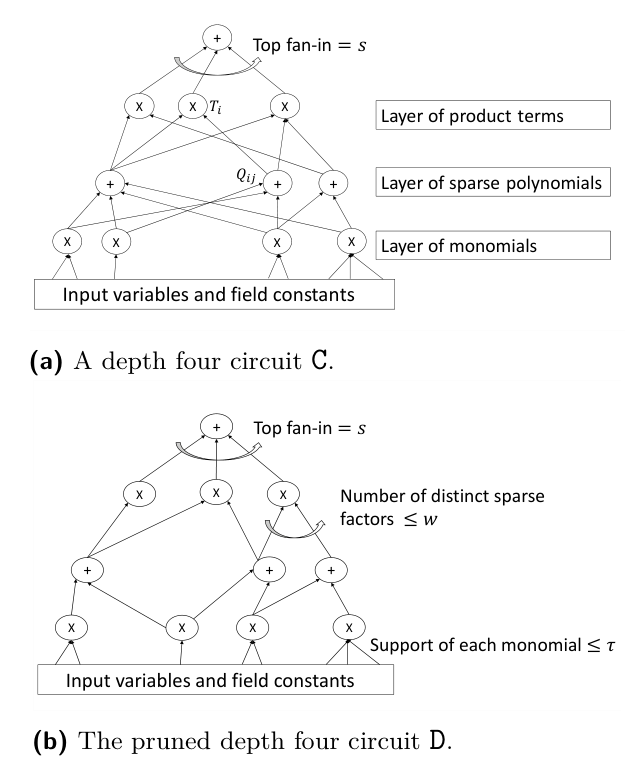
\includegraphics[width=.62\linewidth]{formal-depth4-pruning.png}\\
Figure1:A depth four circuit and its pruned version.\end{center}
\paragraph{Step3:Analysing the measure}
In this step, we analyse the measure $\PSP_{M,k,\ell}$ of the pruned circuit $\mathtt D$, obtained after Steps1 and2, computing a polynomial in the remaining $m$ many $\mathbf x$ and $m$ many $\mathbf y$ variables. More details on this analysis are provided in the following section.
\subsection*{3.1 Upper bound on the measure of a pruned depth four circuit}
Recall the definition of the measure $\PSP_{M,k,\ell}$ from Section2. In Steps1 and2, we will ensure that if a variable $x_i$ is set to a field constant then $y_i$ is also set to a field constant and vice versa. The set $M$ is then the set of indices of the remaining $\mathbf x$ (or $\mathbf y$) variables and $|M|=m$.
\begin{authorclaim}{Lemma7}
Let $\mathtt D$ be a pruned depth four circuit with top fan-in $s$ computing a polynomial in $\mathbf x_M$ and $\mathbf y_M$ variables, where $M\subseteq[3m]$, $|M|=m$. Also, let $d_x,\tau,w$ be as defined earlier, $t=\lfloor d_x/(\ln m)^3\rfloor$, $\delta=1/(\ln m)^2$, $k=\lfloor\delta d_x/t\rfloor$ and $\ell=\lfloor m/(m^{\delta/t}+1)\rfloor$. Then, for sufficiently large $m$,
\[
\PSP_{M,k,\ell}(\mathtt D)\le s\cdot m^{O(1)}\binom m{\ell+2kt\tau}\binom{\lceil w/t\rceil+k-1}{k}.
\]
\end{authorclaim}
We prove the lemma at the end of this section. As $\mathtt D=T_1+\cdots+T_s$, where $T_i$ is a product term and as $\PSP_{M,k,\ell}$ is sub-additive, to prove the lemma it suffices to show that for all $i\in[s]$,
$\PSP_{M,k,\ell}(T_i)\le m^{O(1)}\binom m{\ell+2kt\tau}\binom{\lceil w/t\rceil+k-1}{k}$.
Consider any such product term $T=\prod_{i\in[a]}Q_i^{e_i}$, where $Q_i\in\mathbb F[\mathbf x_M,\mathbf y_M]$, and since $\mathtt D$ is a pruned depth four circuit, $a\le w$. Write $Q_i=Q'_i+Q''_i$, where $Q'_i$ is the sum of all monomials of $Q_i$ wherein the individual degree of every $\mathbf x$ variable is at most two and $Q''_i=Q_i-Q'_i$. Then,
\[
T=\prod_{i\in[a]}(Q'_i+Q''_i)^{e_i}=\prod_{i\in[a]}(Q'_i)^{e_i}+Q'',
\]
where $Q''$ is a polynomial whose every monomial has a $\mathbf x$ variable with degree at least three. Thus, $\PSP_{M,k,\ell}(Q'')=0$ and hence from the sub-additivity of $\PSP_{M,k,\ell}$ we have that
$\PSP_{M,k,\ell}(T)\le\PSP_{M,k,\ell}(\prod_{i\in[a]}(Q'_i)^{e_i})$.
Let $T'=\prod_{i\in[a]}(Q'_i)^{e_i}$. We will now upper bound $\PSP_{M,k,\ell}(T')$. First, we assume without loss of generality that $a=w$ since if $a<w$ then we can multiply with additional sparse polynomials all of which are1. Next we divide the sparse polynomials into disjoint sets such that each set (except perhaps the last) has size exactly $t$. Then, we have that
\[
T'=P_1\cdots P_{\lceil w/t\rceil},\quad\text{where }P_i=\prod_{j=(i-1)t+1}^{\min(it,w)}(Q'_j)^{e_j}.
\]
\begin{authorclaim}{Claim8}
Let $P=(Q'_1)^{e_1}\cdots(Q'_t)^{e_t}$ be one of the polynomials $P_i$. For $k\ge0$, let $P^{(k)}:=\prod_{i\in[t]}(Q'_i)^{\max(e_i-k,0)}$. Then,
$\partial_{\mathbf x}^kP\subseteq\mathbb F\text{-span}\{\mathbf y_M^{\le\infty}\mathbf x_M^{\le k(2t\tau-1)}P^{(k)}\}$.
\end{authorclaim}
The proof of the claim is straighforward and is given in AppendixB.1.
\begin{proof}[Proof of Lemma7]
Recall that it is enough to show the following
\[
\PSP_{M,k,\ell}(T')\le m^{O(1)}\binom m{\ell+2kt\tau}\binom{\lceil w/t\rceil+k-1}{k},
\]
where $T'=P_1\cdots P_{\lceil w/t\rceil}$. Let $v=\lceil w/t\rceil$. Now,
\begin{align*}
\partial_{\mathbf x}^kT'
&\subseteq\mathbb F\text{-span}\{\partial_{\mathbf x}^{k_1}P_1\cdots\partial_{\mathbf x}^{k_v}P_v:k_1+\cdots+k_v=k\}\\
&\subseteq\mathbb F\text{-span}\{\mathbf y_M^{\le\infty}\mathbf x_M^{\le k_1(2t\tau-1)}P_1^{(k_1)}
\cdots\mathbf y_M^{\le\infty}\mathbf x_M^{\le k_v(2t\tau-1)}P_v^{(k_v)}:k_1+\cdots+k_v=k\}\\
&\subseteq\mathbb F\text{-span}\{\mathbf y_M^{\le\infty}\mathbf x_M^{\le k(2t\tau-1)}P_1^{(k_1)}\cdots P_v^{(k_v)}:k_1+\cdots+k_v=k\},
\end{align*}
where the second to last inclusion follows from Claim8. Hence,
\[
\mathbf x_M^\ell\partial_{\mathbf x}^kT'
\subseteq\mathbb F\text{-span}\{\mathbf y_M^{\le\infty}\mathbf x_M^{\le\ell+k(2t\tau-1)}P_1^{(k_1)}\cdots P_v^{(k_v)}:k_1+\cdots+k_v=k\}.
\]
In other words, the space of shifted partials of $T'$ is contained in the $\mathbb F$-span of polynomials of the form $Y\cdot X\cdot P_1^{(k_1)}\cdots P_v^{(k_v)}$ where $Y$ is a monomial in $\mathbf y_M$ variables and $X$ is a monomial in $\mathbf x_M$ variables of degree at most $\ell+k(2t\tau-1)$. Let us analyse the effect of the operations $\sigma_{\mathbf y_M=1}$, $[\cdot]_m$ and $\pi_{\mathbf x}$ on one such polynomial. We will assume that $\deg_{\mathbf y}(Y)\le m$ and $X$ is multilinear for otherwise the polynomial will vanish after the operations are applied. Then, we have that,
\[
\sigma_{\mathbf y_M=1}([\pi_{\mathbf x}(Y\cdot X\cdot P_1^{(k_1)}\cdots P_v^{(k_v)})]_m)
=X\cdot\sigma_{\mathbf y_M=1}([\pi_{\mathbf x}(\sigma_{\operatorname{Supp}(X)=0}(P_1^{(k_1)}\cdots P_v^{(k_v)}))]_{m-\deg(Y)}).
\]
Thus,
\begin{align*}
&\sigma_{\mathbf y_M=1}([\pi_{\mathbf x}(\mathbf x_M^\ell\partial_{\mathbf x}^kT')]_m)\\
&\quad\subseteq\mathbb F\text{-span}\{X\cdot\sigma_{\mathbf y_M=1}([\pi_{\mathbf x}(\sigma_{\operatorname{Supp}(X)=0}(P_1^{(k_1)}\cdots P_v^{(k_v)}))]_i):\\
&\qquad X\text{ is a multilinear monomial in }\mathbf x_M\text{ variables, }\deg(X)\text{ is}\\
&\qquad\text{at most }\ell+k(2t\tau-1),\quad0\le i\le m\text{ and }k_1+\cdots+k_v=k\}.
\end{align*}
Once we fix $i,X$, and $k_1,\ldots,k_v$, $X\cdot\sigma_{\mathbf y_M=1}([\pi_{\mathbf x}(\sigma_{\operatorname{Supp}(X)=0}(P_1^{(k_1)}\cdots P_v^{(k_v)}))]_i)$ is fixed. So,
\begin{align*}
\PSP_{M,k,\ell}(T')
&=\dim\left\langle\sigma_{\mathbf y_M=1}([\pi_{\mathbf x}(\mathbf x_M^\ell\partial_{\mathbf x}^kT')]_m)\right\rangle\\
&\le(m+1)\sum_{j=0}^{\ell+k(2t\tau-1)}\binom mj\binom{v+k-1}k\\
&\le(m+1)(\ell+2kt\tau)\binom m{\ell+2kt\tau}\binom{v+k-1}k\\
&=m^{O(1)}\binom m{\ell+2kt\tau}\binom{\lceil w/t\rceil+k-1}k,
\end{align*}
where the second last inequality follows from Claim9 (proved in AppendixB.1).
\end{proof}
\begin{authorclaim}{Claim9}
Let $\ell,k,t$ and $\tau$ be as defined earlier. Then, $\ell+2kt\tau<m/2$.
\end{authorclaim}

\subsection*{3.2 Pruning a depth four circuit}
As mentioned before, we will prune the circuit $\mathtt C$ computing $f_n$ in two steps--first we will restrict the bottom support of $\mathtt C$ and then we will get rid of all heavy gates in it.
\subsection*{3.2.1 Step1--Restricting the bottom support of $\mathtt C$}
If the number of monomials in $\mathtt C$ is more than $\lfloor m^2d_x/(\ln m)^5\rfloor$, there is nothing to prove. Otherwise, we show that we can get rid of all monomials with support more than $\tau=\lfloor20\ln m\rfloor$.
\begin{authorclaim}{Lemma10}
Let the number of monomials in $\mathtt C$ be at most $\lfloor m^2d_x/(\ln m)^5\rfloor$. Then, for sufficiently large $m$, there exists $M_1\subseteq[3m]$, $|M_1|=m$ such that all monomials in $\mathtt C_1$ obtained from $\mathtt C$ by setting variables $\mathbf x_{M_1}$ and $\mathbf y_{M_1}$ to 0 have support at most $\tau$.
\end{authorclaim}
\begin{proof}
We first present a greedy procedure to remove all monomials with support more than $\tau$ and then argue that it sets $m$ variables each from $\mathbf x$ and $\mathbf y$ to 0. In each iteration the procedure picks a pair of variables that appears in a large number of monomials with support more than $\tau$ and set them to 0.
\begin{authorclaim}{Procedure1:Restriction procedure}
\begin{enumerate}
\item $M_1\leftarrow\varnothing$, $\mathtt C_1\leftarrow\mathtt C$, $H:=$ set of all monomials of $\mathtt C_1$ with support more than $\tau$.
\item For $j\in[3m]$, $e(j):=$ number of monomials in $H$ containing $x_j$ or $y_j$.
\item while $H\ne\varnothing$ do
\item Pick $j'\in[3m]\setminus M_1$ such that $e(j')\ge e(j)$ for all $j\in[3m]$. Set $x_{j'}=0$ and $y_{j'}=0$. Update $M_1\leftarrow M_1\cup\{j'\}$, $\mathtt C_1\leftarrow$ circuit obtained from $\mathtt C_1$ by setting $x_{j'}$ and $y_{j'}$ to 0, $H\leftarrow$ set of all monomials of $\mathtt C_1$ with support more than $\tau$, and $e(j)\leftarrow$ number of monomials in $H$ containing $x_j$ or $y_j$.
\item end while
\end{enumerate}
\end{authorclaim}
It is clear that the bottom support of $\mathtt C_1$ obtained after the termination of the procedure is at most $\tau$. Also, since we are only setting variables to 0, it trivially follows that the procedure does not increase the number of gates nor does it increase the fan-in of any gate in the circuit. Claim11 (proved in AppendixB.2) implies that the procedure terminates in at most $m$ iterations. If it terminates before $m$ iterations, we arbitrarily add an appropriate number of $j\in[3m]$ to $M_1$ so that $|M_1|=m$ and set $x_j$ and $y_j$ to 0 for all such $j$.
\end{proof}
\begin{authorclaim}{Claim11}
Procedure1 terminates in at most $m$ iterations.
\end{authorclaim}
\paragraph{Remark}
Procedure1 looks similar to an approximation algorithm for the Set Cover problem [102] (Section1.2,page6). This is because the problem of removing monomials with support more than $\tau$ can be formulated as an instance of Set Cover with the universe being all such monomials and with a set corresponding to each $j\in[3m]$. For a $j\in[3m]$, the corresponding set will contain all monomials with support more than $\tau$ in which at least one of $x_j$ and $y_j$ appears.
\subsection*{3.2.2 Step2--Pruning the heavy gates from $\mathtt C_1$}
A sparse polynomial $Q$ in $\mathtt C_1$ is said to be light if its fan-in is at most $m/(\ln m)^2$, i.e., at most $m/(\ln m)^2$ many non-zero monomials are present in $Q$. If the sum of fan-ins of all the light sparse polynomials is $\Omega(m^2d_x/(\ln m)^5)$ then there is nothing to prove. So assume that the sum of fan-ins of all the light sparse polynomials is $O(m^2d_x/(\ln m)^5)$. Recall that a product term is called heavy if it has at least $w=\lfloor md_x/(\lambda_0(\ln m)^3)\rfloor$ many distinct sparse polynomials connected to it (where $\lambda_0$ is a large enough constant fixed in AppendixC). Observe that one of the following cases is true:
\begin{enumerate}
\item There is a heavy gate in $\mathtt C_1$, that is connected to at most $md_x/(2\lambda_0(\ln m)^3)$ light sparse polynomials.
\item Every heavy gate is connected to at least $md_x/(2\lambda_0(\ln m)^3)$ light sparse polynomials.
\end{enumerate}
Case1 clearly implies a lower bound of $\Omega(m^2d_x/(\ln m)^5)$. Else, we prove the following lemma.
\begin{authorclaim}{Lemma12}
Let $\mathtt C_1$ be the circuit (obtained from Lemma10) having at most $m$ heavy gates such that every heavy gate is connected to at least $md_x/(2\lambda_0(\ln m)^3)$ light sparse polynomials, and the sum of fan-ins of all the light sparse polynomials is at most $m^2d_x/(160\lambda_0(\ln m)^5)$. Then, there exist $M_2\subseteq[3m]\setminus M_1$, $|M_2|=m$ and $\alpha_l,\beta_l\in\mathbb F$ for $l\in M_2$, such that setting $x_l=\alpha_l$, $y_l=\beta_l$ for all $l\in M_2$ removes all heavy gates from $\mathtt C_1$.
\end{authorclaim}
\begin{proof}
We first present the pruning procedure and then argue its correctness. For any light sparse polynomial $Q_j$ in $\mathtt C_1$, let $b_j$ and $c_j$ be equal to the fan-in of $Q_j$ and the number of distinct heavy gates connected to $Q_j$ in $\mathtt C_1$ respectively. As $Q_j$ is a light sparse polynomial, $b_j\le m/(\ln m)^2$. In this procedure, while all the heavy gates do not disappear from $\mathtt C_1$, we pick a sparse polynomial whose ratio of the number of distinct heavy gates connected to it and fan-in is maximum and set that to zero by evaluating it to one of its roots in $\mathbb F$. This can be done as $\mathbb F$ is algebraically closed. The restricted support of the monomials in $\mathtt C_1$ ensure that at the end of this procedure, only a small fraction of the variables are set.
\begin{authorclaim}{Procedure2:Pruning heavy gates from $\mathtt C_1$}
\begin{enumerate}
\item Set $i=1$ and $M_2=\varnothing$. Let $s_1\le m$ be the number of heavy gates in $\mathtt C_1$. Choose a non-constant light sparse polynomial $Q_1$ from $\mathtt C_1$ such that the ratio $c_1/b_1$ is maximum and add the indices of the variables appearing in $Q_1$ to $M_2$. As $b_1\le m/(\ln m)^2$, we have $\tau b_1\le m$.
\item Make $Q_1$ equal to zero by setting at most $\tau b_1$ many variables appearing in $Q_1$ to field constants. By doing so, at least $c_1$ many heavy gates vanish from $\mathtt C_1$.
\item while $(\tau(b_1+\cdots+b_i)\le m)$ do
\item Increment $i$ by 1.
\item Let $s_i$ be the number of heavy gates in the current circuit $\mathtt C_1$ obtained after the $(i-1)$-th iteration. Clearly, $s_i\le s_{i-1}-c_{i-1}$. If $s_i=0$ then exit the loop.
\item Otherwise, choose a non-constant light sparse polynomial $Q_i$ from $\mathtt C_1$ having the maximum value of $c_i/b_i$ in $\mathtt C_1$ and add the indices of the variables appearing in $Q_i$ to $M_2$.
\item Make $Q_i$ equal to zero by setting at most $\tau b_i$ many variables appearing in $Q_i$ to field constants. By doing so, at least $c_i$ many heavy gates vanish from $\mathtt C_1$.
\item end while
\end{enumerate}
\end{authorclaim}
\begin{authorclaim}{Claim13}
Let $\overline M_1=[3m]\setminus M_1$. Procedure2 sets at most $m$ many variables in $\mathbf x_{\overline M_1}\cup\mathbf y_{\overline M_1}$ to field constants and removes all the heavy gates from $\mathtt C_1$.
\end{authorclaim}
The above claim is proved in AppendixB.3. The claim implies that $|M_2|\le m$. If $|M_2|<m$, add appropriate number of elements from $[3m]\setminus M_1\cup M_2$ to $M_2$ arbitrarily so that $|M_2|=m$. For every $l\in M_2$, if $x_l$ or $y_l$ is not set to a field constant then set $x_l=0$ or $y_l=0$ respectively. Clearly, we end up setting exactly $m$ variables each from $\mathbf x_{\overline M_1}$ and $\mathbf y_{\overline M_1}$.
\end{proof}
\paragraph{Remark}
Procedure2 resembles an approximation algorithm for the Weighted Set Cover problem [99] (Section2.1,page16). This is no coincidence as the problem of removing heavy gates can be formulated as an instance of Weighted Set Cover with the universe being all heavy gates and with a set corresponding to every sparse polynomial $Q$. The set corresponding to $Q$ contains all heavy gates connected to $Q$ and has a cost equal to the number of monomials feeding into $Q$.

\section*{4 An explicit polynomial family with high measure}
We now describe the family $\{f_n\}_{n\ge1}$, whose $n$-th member $f_n$ is a polynomial in variables $\mathbf x=\{x_1,\ldots,x_{3m}\}$ and $\mathbf y=\{y_1,\ldots,y_{3m}\}$, where $m\in[n/2,2n]$ will be fixed later.
\[
f_n:=\sum_{\substack{S\subseteq[3m]\\|S|=m}}\left(\prod_{i\in S}y_i\right)\cdot\operatorname{NW}_r(\mathbf x_S),
\]
where $\operatorname{NW}_r$ is a variant of the Nisan-Wigderson design polynomial (introduced in [52]), the construction of which is described later and $r$ is a parameter fixed in this construction. Note that $\{f_n\}_{n\ge1}$ is in VNP. Given a monomial, in order to find its coefficient in $f_n$, we first check if the monomial is multilinear and of degree $m$ in $\mathbf y$ variables. If it is so and $S$ is the set of the indices of the $m$ many $\mathbf y$ variables in the monomial then simply return the coefficient of the part of the monomial in $\mathbf x$ variables in $\operatorname{NW}_r(\mathbf x_S)$--this can be done as the Nisan-Wigderson polynomial family is in VNP.
Let $M_1$ and $M_2$ be as in Section3 and $M=[3m]\setminus(M_1\cup M_2)$. Let $f_1$ be the polynomial computed by the pruned circuit $\mathtt D$, which is obtained from $f=f_n$ by setting the variables $\mathbf x_{\overline M}$ and $\mathbf y_{\overline M}$ to field constants as in Section3.2. Let us now see how $\PSP_{M,k,\ell}(f_1)$ is related to $\dim\langle\pi_{\mathbf x}(\mathbf x_M^\ell\partial_{\mathbf x}^k\operatorname{NW}_r)\rangle$.
\begin{authorclaim}{Lemma14}
Let $f_1$ be as defined above. Then,
$\PSP_{M,k,\ell}(f_1)=\dim\langle\pi_{\mathbf x}(\mathbf x_M^\ell\partial_{\mathbf x}^k\operatorname{NW}_r(\mathbf x_M))\rangle$.
\end{authorclaim}
\begin{proof}
The proof follows easily from the following two observations:
\begin{enumerate}
\item The two operations in $\mathbf y$ variables and the three operations in $\mathbf x$ variables (in the definition of $\PSP_{M,k,\ell}$) commute. That is, we have
\[
\sigma_{\mathbf y_M=1}([\pi_{\mathbf x}(\mathbf x_M^\ell\partial_{\mathbf x}^kf_1)]_m)
=\pi_{\mathbf x}(\mathbf x_M^\ell\partial_{\mathbf x}^k(\sigma_{\mathbf y_M=1}([f_1]_m))).
\]
\item $f_1=(\prod_{i\in M}y_i)\cdot\operatorname{NW}_r(\mathbf x_M)+f'$, where $f'\in\mathbb F[\mathbf x_M,\mathbf y_M]$ and $\deg_{\mathbf y}(f')<m$.
\end{enumerate}
From these observations we have that
\begin{align*}
\PSP_{M,k,\ell}(f_1)
&=\dim\left\langle\sigma_{\mathbf y_M=1}([\pi_{\mathbf x}(\mathbf x_M^\ell\partial_{\mathbf x}^kf_1)]_m)\right\rangle\\
&=\dim\left\langle\pi_{\mathbf x}\left(\mathbf x_M^\ell\partial_{\mathbf x}^k
\left(\sigma_{\mathbf y_M=1}\left[\left(\prod_{i\in M}y_i\right)\operatorname{NW}_r(\mathbf x_M)+f'\right]_m\right)\right)\right\rangle\\
&=\dim\left\langle\pi_{\mathbf x}(\mathbf x_M^\ell\partial_{\mathbf x}^k\operatorname{NW}_r(\mathbf x_M))\right\rangle.
\end{align*}
The last equality follows from the fact that
$\sigma_{\mathbf y_M=1}([(\prod_{i\in M}y_i)\cdot\operatorname{NW}_r(\mathbf x_M)+f']_m)=\operatorname{NW}_r(\mathbf x_M)$.
\end{proof}
\paragraph{Construction of $\operatorname{NW}_r$}
Let $d_x=\lfloor\sqrt n/\ln n\rfloor$. Pick an $\alpha$ such that $d_x\lceil d_x^{1+\alpha}\rceil\le n\le2d_x\lceil d_x^{1+\alpha}\rceil$;this forces $\alpha$ to be $\Theta(\ln\ln n/\ln n)$. Let $q$ be a prime number between $\lceil d_x^{1+\alpha}\rceil$ and $2\lceil d_x^{1+\alpha}\rceil$--such a prime exists [26]--and let $m=d_xq$. Thus, $d_x\lceil d_x^{1+\alpha}\rceil\le m\le2d_x\lceil d_x^{1+\alpha}\rceil$ and hence $n/2\le m\le2n$;moreover, it can be easily verified that $d_x\in[\sqrt m/(2\sqrt2\ln m),2\sqrt2\sqrt m/\ln m]$;both being as required in Section3. Also notice that this means $q=\Theta(\sqrt n\ln n)$. Let $\beta=1/\ln m$ and $r=\lfloor((\alpha+\beta)/(2(1+\alpha)))d_x\rfloor-1$, $\mathbf u=(u_{1,1},\ldots,u_{1,q},\ldots,u_{d_x,1},\ldots,u_{d_x,q})$ and define
\[
\operatorname{NW}_r(\mathbf u):=\sum_{\substack{h(z)\in\mathbb F_q[z]\\\deg(h)\le r}}u_{1,h(1)}\cdots u_{d_x,h(d_x)}.
\]
A lower bound on $\dim\langle\pi_{\mathbf x}(\mathbf x_M^\ell\partial_{\mathbf x}^k\operatorname{NW}_r)\rangle$ was proved in [51,85]. Since their analysis continues to hold for our choice of parameters--which only slightly differ from the parameters in [85]--we omit the proof of the following theorem. Moreover, while they prove this lower bound over fields of characteristic zero, the same proof also works if the characteristic is greater than
$q^{(r+1)\cdot\min\{\binom mk\binom m\ell,\binom m{\ell-d_x-k}\}}$.
\begin{authorclaim}{Theorem15 (Lemma5.2 of [51],Lemma4.1 of [85])}
\[
\dim\left\langle\pi_{\mathbf x}(\mathbf x_M^\ell\partial_{\mathbf x}^k\operatorname{NW}_r(\mathbf x_M))\right\rangle
\ge\frac1{m^{O(1)}}\min\left\{\frac1{4^k}\binom m\ell\binom mk,\binom m{\ell+d_x-k}\right\}.
\]
\end{authorclaim}
Hence, from Lemma14 and Theorem15 we get
\begin{authorclaim}{Lemma16}
$\PSP_{M,k,\ell}(f_1)\ge m^{-O(1)}\min\{4^{-k}\binom m\ell\binom mk,\binom m{\ell+d_x-k}\}$.
\end{authorclaim}

\section*{5 Proof of Theorem1}
As before, let $\mathtt C$ be a depth four circuit computing the polynomial $f_n$. Before proving the theorem, let us first justify the assumption that $\mathbb F$ is an algebraically closed field that we made in Section3. Suppose not. Then, let $\overline{\mathbb F}$ be its algebraic closure. Since $\mathtt C$ is also a circuit over $\overline{\mathbb F}$ and $f_n$ a polynomial over $\overline{\mathbb F}$, we can make all arguments assuming the underlying field to be $\overline{\mathbb F}$. Since the size of a circuit does not depend on the underlying field, the lower bound so obtained will continue to hold when we treat $\mathtt C$ as a circuit over $\mathbb F$.
First we will prove a lower bound on the number of wires of $\mathtt C$. If the number of monomials in $\mathtt C$ is $\lfloor m^2d_x/(\ln m)^5\rfloor$ then there is nothing to prove. Otherwise from Lemma10, we can obtain a circuit $\mathtt C_1$ such that the support of all the monomials of $\mathtt C_1$ is at most $\tau=\lfloor20\ln m\rfloor$, the number of gates in $\mathtt C_1$ is at most the number of gates in $\mathtt C$ and the fan-in of each gate in $\mathtt C_1$ is upper bounded by the fan-in of the corresponding gate in $\mathtt C$. Then, if $\mathtt C_1$ does not satisfy the hypothesis of Lemma12, the size of $\mathtt C_1$ and hence the size of $\mathtt C$ is at least $\Omega(m^2d_x/(\ln m)^5)$. Otherwise, we can obtain a pruned circuit $\mathtt D$ such that the top fan-in and the bottom support of $\mathtt D$ are upper bounded by the top fan-in and bottom support of $\mathtt C_1$ and so proving a lower bound on the top fan-in of $\mathtt D$ would suffice.
As $\mathtt D$ computes $f_1$ (defined in Section4), $\PSP_{M,k,\ell}(\mathtt D)=\PSP_{M,k,\ell}(f_1)$. Lemma7 and 16 imply
\begin{equation}
s\ge\frac{m^{-O(1)}\min\{4^{-k}\binom m\ell\binom mk,\binom m{\ell+d_x-k}\}}
{m^{O(1)}\binom m{\ell+2kt\tau}\binom{\lceil w/t\rceil+k-1}k},\tag{1}
\end{equation}
and the required lower bound follows from the next claim, which is proved in AppendixC.
\begin{authorclaim}{Claim17}
The top fan-in $s$ of $\mathtt D$ is $\omega(m^2d_x/(\ln m)^5)$.
\end{authorclaim}
Now let us prove the lower bound on the number of gates. Notice that if the circuit $\mathtt C$ computing $f$ has a heavy gate as defined in Section3 then we are done. So assume that it does not have any heavy gates. Now, if the number of monomials in $\mathtt C$ is $\lfloor m^2d_x/(\ln m)^5\rfloor$ then there is nothing to prove. Otherwise from Lemma10, we can obtain a circuit $\mathtt C_1$ such that the support of all the monomials of $\mathtt C_1$ is at most $\tau=\lfloor20\ln m\rfloor$, the number of gates in $\mathtt C_1$ is at most the number of gates in $\mathtt C$ and the fan-in of each gate in $\mathtt C_1$ is upper bounded by the fan-in of the corresponding gate in $\mathtt C$. Obtain a circuit $\mathtt D$ from $\mathtt C_1$ by picking a set $M_2\subseteq[3m]\setminus M_1$ (where $M_1$ is as in Lemma10), $|M_2|=m$ arbitrarily and setting variables in $\mathbf x_{M_2}$ and $\mathbf y_{M_2}$ to 0 (notice that the top fan-in and bottom support of $\mathtt D$ are upper bounded by the top fan-in and bottom support of $\mathtt C_1$). Now $\mathtt D$ computes $f_1$ (where $f_1$ is as defined in Section4) and just as it was done in the preceding paragraph, we can show that the top fan-in of $\mathtt D$ is $\omega(m^2d_x/(\ln m)^5)$. However, we only get an $\Omega(md_x/(\ln m)^3)$ lower bound on the number of gates since the definition of a heavy gate is the bottleneck.

\section*{B Missing proofs from Section3}
\subsection*{B.1 Proofs from Section3.1}
\begin{authorclaim}{Claim8}
Let $P=(Q'_1)^{e_1}\cdots(Q'_t)^{e_t}$ be one of the polynomials $P_i$. For $k\ge0$, let $P^{(k)}:=\prod_{i\in[t]}(Q'_i)^{\max(e_i-k,0)}$. Then, $\partial_{\mathbf x}^kP\subseteq\mathbb F\text{-span}\{\mathbf y_M^{\le\infty}\mathbf x_M^{\le k(2t\tau-1)}P^{(k)}\}$.
\end{authorclaim}
\begin{proof}
We prove the claim by induction on $k$. If $k=0$, then $\partial_{\mathbf x_M}^0P=\{P\}=\{P^{(0)}\}$ and hence the claim is true. Assume that the claim is true for $k$. Let $X$ be a multilinear monomial of degree $k+1$ in $\mathbf x$ variables. Then $X=xX'$ where $X'$ is a multilinear monomial of degree $k$ in $\mathbf x$ variables and $x$ one of the $\mathbf x$ variables. From the induction hypothesis we have that,
\[
\frac{\partial P}{\partial X'}=g\cdot P^{(k)}
\]
where $g$ is a polynomial in $\mathbb F[\mathbf x_M,\mathbf y_M]$ with $\mathbf x_M$ degree of $g$ being at most $k(2t\tau-1)$ while its $\mathbf y_M$ degree can be arbitrarily large.
Let $J:=\{j\in[t]:e_j>k\}$. We have that,
\begin{align*}
\frac{\partial P}{\partial X}
&=\frac{\partial}{\partial x}(g\cdot P^{(k)})
=\frac{\partial}{\partial x}\left(g\cdot\prod_{j\in J}(Q'_j)^{e_j-k}\right)\\
&=\frac{\partial g}{\partial x}\prod_{j\in J}(Q'_j)^{e_j-k}
+g\sum_{j\in J}(e_j-k)(Q'_j)^{e_j-k-1}\frac{\partial Q'_j}{\partial x}
\prod_{i\in J\setminus\{j\}}(Q'_i)^{e_i-k}\\
&=\left(\frac{\partial g}{\partial x}\prod_{j\in J}Q'_j
+g\sum_{j\in J}(e_j-k)\frac{\partial Q'_j}{\partial x}
\prod_{i\in J\setminus\{j\}}Q'_i\right)
\prod_{j\in J}(Q'_j)^{e_j-k-1}.
\end{align*}
Observe that as $\mathtt D$ is a pruned depth four circuit, the support of all monomials of $Q'_j$ is upper bounded by $\tau$ and as in any monomial the individual degree of any $\mathbf x$ variable is at most two, $\deg_{\mathbf x}(Q'_j)\le2\tau$. Also, $|J|\le t$ and hence
\[
\deg_{\mathbf x}\left(\frac{\partial g}{\partial x}\prod_{j\in J}Q'_j
+g\sum_{j\in J}(e_j-k)\frac{\partial Q'_j}{\partial x}
\prod_{i\in J\setminus\{j\}}Q'_i\right)\le(k+1)(2t\tau-1).
\]
As $\prod_{j\in J}(Q'_j)^{e_j-k-1}=P^{(k+1)}$, the claim is true for $k+1$.
\end{proof}
\begin{authorclaim}{Claim9}
Let $\ell,k,t$ and $\tau$ be as defined earlier. Then, $\ell+2kt\tau<m/2$.
\end{authorclaim}
\begin{proof}
We will show that the ratio $(m/2-2kt\tau)/\ell>1$. Putting the values of $k$ and $\ell$,
\[
\frac{m/2-2kt\tau}{\ell}
=\frac{m/2-2\lfloor\delta d_x/t\rfloor t\tau}{\lfloor m/(m^{\delta/t}+1)\rfloor}
\ge\left(\frac12-\frac{2\delta d_x\tau}{m}\right)(m^{\delta/t}+1).
\]
So, we need to show that
\begin{align*}
\frac1{1/2-2\delta d_x\tau/m}<m^{\delta/t}+1
&\Longleftrightarrow\frac1{1/2-2\delta d_x\tau/m}-1<m^{\delta/t}\\
&\Longleftrightarrow\frac{1+4\delta d_x\tau/m}{1-4\delta d_x\tau/m}<m^{\delta/t}.
\end{align*}
For large enough $m$, $4\delta d_x\tau/m\le1/2$. Using $1+x\le e^x$, which holds for all $x\in\mathbb R$, and $1/(1-x)\le e^{2x}$, which holds for $0\le x\le1/2$ we get:
\[
\frac{1+4\delta d_x\tau/m}{1-4\delta d_x\tau/m}\le e^{12\delta d_x\tau/m}.
\]
So showing that $e^{12\delta d_x\tau/m}<m^{\delta/t}$ would suffice. Now,
$e^{12\delta d_x\tau/m}<m^{\delta/t}\Longleftrightarrow e^{12d_xt\tau/m}<m$.
Putting the values of $d_x,t$ an $\tau$, we get that
\[
\frac{12d_xt\tau}{m}
=\frac{12d_x\lfloor d_x/(\ln m)^3\rfloor\lfloor20\ln m\rfloor}{m}
\le\frac{12d_x^2\cdot20\ln m}{m(\ln m)^3}
=\Theta\left(\frac m{m(\ln m)^2(\ln m)^2}\right)
=\Theta\left(\frac1{(\ln m)^4}\right)=o(1)
\]
as $d_x=\Theta(\sqrt m/\ln m)$. Thus $e^{12d_xt\tau/m}<m$.
\end{proof}
\subsection*{B.2 Proof from Section3.2.1}
\begin{authorclaim}{Claim11}
Procedure1 terminates in at most $m$ iterations.
\end{authorclaim}
\begin{proof}
Let $H_i$ be the set $H$ after the $i$-th iteration of the procedure. Since each monomial in $H_i$ has support more than $\tau$, for any such monomial there are at least $\tau/2$ distinct $j\in[3m]\setminus M_1$ such that at least one of $x_j$ and $y_j$ appears in it. Counting the number of times at least one of $x_j$ and $y_j$ appears in a monomial in $H_i$ and summing up these counts for all $j\in[3m]\setminus M_1$, we get that
\[
\sum_{j\in[3m]\setminus M_1}e(j)\ge\tau|H_i|/2;
\]
so from an averaging argument there exists a $j$ such that $e(j)\ge\tau|H_i|/(6m)$.
Hence, the size of $H_{i+1}$ is upper bounded as $|H_{i+1}|\le|H_i|(1-\tau/(6m))$.
So after $i$ iterations of the procedure we get,
\begin{align*}
|H_i|&\le|H_0|(1-\tau/(6m))^i\\
&\le\lfloor m^2d_x/(\ln m)^5\rfloor(1-\lfloor20\ln m\rfloor/(6m))^i\\
&\le\frac{m^2d_x}{(\ln m)^5}(1-(20\ln m-1)/(6m))^i\\
&\le\frac{m^2d_x}{(\ln m)^5}e^{-3i\ln m/m}\quad(\text{for sufficiently large }m)\\
&=\frac{m^2d_x}{(\ln m)^5}m^{-3i/m}.
\end{align*}
For $i=m$, $|H_i|<1$ (for sufficiently large $m$), i.e., the procedure terminates in at most $m$ iterations.
\end{proof}
\subsection*{B.3 Proof from Section3.2.2}
\begin{authorclaim}{Claim13}
Let $\overline M_1=[3m]\setminus M_1$. Procedure2 sets at most $m$ many variables in $\mathbf x_{\overline M_1}\cup\mathbf y_{\overline M_1}$ to field constants and removes all the heavy gates from $\mathtt C_1$.
\end{authorclaim}
\begin{proof}
In each iteration, we evaluate a light sparse polynomial in $\mathtt C_1$ to zero. This can be done as $\mathbb F$ is an algebraically closed field. Since the support of every monomial in $\mathtt C_1$ is at most $\tau$, we end up setting at most $\tau m/(\ln m)^2\le20m/\ln m$ many variables to field constants in each iteration. As we can afford to set $m$ variables, Step2 of the procedure executes successfully. For some $i\in\mathbb N$, the while loop terminates in the $i$-th iteration in either of the following two cases:
\begin{enumerate}
\item All the heavy gates get eliminated after the $(i-1)$-th iteration, i.e., $s_i=0$.
\item $\tau(b_1+\cdots+b_i)>m$. (We show in the following subclaim that all the heavy gates are eliminated before this happens. Hence, the procedure stops only in the above case.)
\end{enumerate}
\begin{authorclaim}{Subclaim18}
Let $i\in\mathbb N$ be such that $\tau(b_1+\cdots+b_{i-1})\le m$ but $\tau(b_1+\cdots+b_i)>m$. Then, all the heavy gates in $\mathtt C_1$ get eliminated in the first $(i-1)$ iterations of Procedure2.
\end{authorclaim}
If we assume Subclaim18 then Claim13 is proved.
\end{proof}
\begin{proof}[Proof of Subclaim18]
For $1\le j<i$, let $(Q_{j,1},\ldots,Q_{j,r_j})$ be the available light sparse polynomials in $\mathtt C_1$ after the $(j-1)$-th iteration. Recall that $s_j$ is the number of heavy gates in $\mathtt C_1$ after the $(j-1)$-th iteration. Suppose, $s_j\ge1$ (otherwise, we have nothing to prove). For every $l\in[r_j]$, $b_{j,l}$ and $c_{j,l}$ refer to the fan-in of $Q_{j,l}$ and the number of distinct heavy gates connected to $Q_{j,l}$ in $\mathtt C_1$ respectively. We may assume that $b_{j,l}\ne0$ for every $l\in[r_j]$. It is given that
\begin{equation}
b_{j,1}+\cdots+b_{j,r_j}\le\frac{m^2d_x}{160\lambda_0(\ln m)^5}.\tag{2}
\end{equation}
Since every heavy gate is connected to at least $md_x/(2\lambda_0(\ln m)^3)$ many light sparse polynomials in $\mathtt C_1$,
\[
s_j\frac{md_x}{2\lambda_0(\ln m)^3}\le c_{j,1}+\cdots+c_{j,r_j}.
\]
As $b_{j,1},\ldots,b_{j,r_j}$ are all non-zero, we get
\[
s_j\frac{md_x}{2\lambda_0(\ln m)^3}
\le\frac{c_{j,1}}{b_{j,1}}b_{j,1}+\cdots+\frac{c_{j,r_j}}{b_{j,r_j}}b_{j,r_j}.
\]
Let $u\in[r_j]$ be such that $c_{j,u}/b_{j,u}=\max\{c_{j,1}/b_{j,1},\ldots,c_{j,r_j}/b_{j,r_j}\}$. Let $c_j:=c_{j,u}$ and $b_j:=b_{j,u}$. Then, the above equation implies
\[
s_j\frac{md_x}{2\lambda_0(\ln m)^3}\le\frac{c_j}{b_j}(b_{j,1}+\cdots+b_{j,r_j}).
\]
From Equation(2), we get that for every $1\le j<i$,
\[
s_j\frac{md_x}{2\lambda_0(\ln m)^3}
\le\frac{c_j}{b_j}\frac{m^2d_x}{160\lambda_0(\ln m)^5},
\]
which implies
\begin{equation}
\frac{80s_jb_j(\ln m)^2}{m}\le c_j.\tag{3}
\end{equation}
Thus, by setting the light sparse polynomial $Q_{j,u}$ to zero in the $j$-th iteration, we get rid of at least $80s_jb_j(\ln m)^2/m$ many heavy gates from $\mathtt C_1$. Recall that $s_{j+1}$ is the number of available heavy gates after the $j$-th iteration. Then, for every $1\le j<i$,
\begin{equation}
s_{j+1}\le s_j-c_j\le s_j(1-80b_j(\ln m)^2/m).\tag{4}
\end{equation}
Hence, for every $1\le j<i$,
\begin{equation}
s_{j+1}\le s_1\prod_{l=1}^j(1-80b_l(\ln m)^2/m).\tag{5}
\end{equation}
Also, for every $l\le j$, we have $c_l\le s_l$. Thus, Equation(3) implies
\begin{equation}
80b_l(\ln m)^2/m\le1.\tag{6}
\end{equation}
As $1-a\le e^{-a/2}$ for $0\le a\le1$, Equations(5) and(6) imply
\begin{equation}
s_{j+1}\le s_1\prod_{l=1}^je^{-40b_l(\ln m)^2/m}
=s_1e^{-40(b_1+\cdots+b_j)(\ln m)^2/m}.\tag{7}
\end{equation}
It is given that $\tau(b_1+\cdots+b_i)>m$, which implies $\tau(b_1+\cdots+b_{i-1})>m-\tau b_i$. As $b_i$ is the fan-in of a light sparse polynomial, $b_i\le m/(\ln m)^2$ and so
\begin{equation}
\tau(b_1+\cdots+b_{i-1})>m-\frac{m\tau}{(\ln m)^2}.\tag{8}
\end{equation}
On substituting $j=i-1$, $\tau=\lfloor20\ln m\rfloor$ and the value of $\tau(b_1+\cdots+b_{i-1})$ from Equation(8) in Equation(7), we get
\[
s_i\le s_1\exp\left(-\frac{40(\ln m)^2}{m}
\left(\frac m{20\ln m}-\frac m{(\ln m)^2}\right)\right)
=s_1e^{-(2\ln m-40)}.
\]
For large enough $m$, $s_i\le s_1/m^{1.9}$. Since $s_1\le m$, we get $s_i=0$ (as it is a natural number). In other words, we get rid of all the heavy gates within $(i-1)$ iterations.
\end{proof}

\section*{C Missing proofs from Section5}
\begin{authorclaim}{Claim17}
The top fan-in $s$ of $\mathtt D$ is $\omega(m^2d_x/(\ln m)^5)$.
\end{authorclaim}
\begin{proof}
From Equation(1), we have
\begin{align*}
s&\ge\frac{m^{-O(1)}\min\{4^{-k}\binom m\ell\binom mk,\binom m{\ell+d_x-k}\}}
{m^{O(1)}\binom m{\ell+2kt\tau}\binom{\lceil w/t\rceil+k-1}k}\\
&\ge\frac1{m^{O(1)}\binom{\lceil w/t\rceil+k-1}k}
\min\left\{\frac{\binom mk}{4^k}\frac{\binom m{\ell+1}}{\binom m{\ell+2kt\tau+1}},
\frac{\binom m{\ell+d_x-k}}{\binom m{\ell+2kt\tau}}\right\}\\
&=\frac1{m^{O(1)}\binom{\lceil w/t\rceil+k-1}k}
\min\left\{\begin{aligned}
&\frac{\binom mk}{4^k}\frac{(m-\ell-2kt\tau-1)!}{(m-\ell-1)!}
\frac{(\ell+2kt\tau+1)!}{(\ell+1)!},\\
&\frac{(m-\ell-2kt\tau)!}{(m-\ell-d_x+k)!}
\frac{(\ell+2kt\tau)!}{(\ell+d_x-k)!}
\end{aligned}\right\}\\
&=\frac1{m^{O(1)}\binom{\lceil w/t\rceil+k-1}k}
\min\left\{\begin{aligned}
&\frac{\binom mk}{4^k}
e^{(-2kt\tau)\ln((m-\ell-1)/(\ell+1))\pm o(1)},\\
&e^{(d_x-2kt\tau-k)\ln((m-\ell)/\ell)\pm o(1)}
\end{aligned}\right\}\quad(\text{Using Proposition5.})\\
&\ge\frac1{m^{O(1)}\binom{\lceil w/t\rceil+k-1}k}
\min\left\{\frac{\binom mk}{4^k}\left(\frac m{\ell+1}-1\right)^{-2kt\tau},
\left(\frac m\ell-1\right)^{d_x-2kt\tau-k}\right\}\\
&=\frac1{m^{O(1)}\binom{\lceil w/t\rceil+k-1}k}
\min\left\{\begin{aligned}
&\frac{\binom mk}{4^k}
\left(\frac m{\lfloor m/(m^{\delta/t}+1)\rfloor+1}-1\right)^{-2kt\tau},\\
&\left(\frac m{\lfloor m/(m^{\delta/t}+1)\rfloor}-1\right)^{d_x-2kt\tau-k}
\end{aligned}\right\}\\
&\ge\frac1{m^{O(1)}\binom{\lceil w/t\rceil+k-1}k}
\min\left\{\frac{\binom mk}{4^k}\left(\frac m{m/(m^{\delta/t}+1)}-1\right)^{-2kt\tau},
\left(\frac m{m/(m^{\delta/t}+1)}-1\right)^{d_x-2kt\tau-k}\right\}\\
&\ge\frac1{m^{O(1)}\binom{\lceil w/t\rceil+k-1}k}
\min\left\{\frac{\binom mk}{4^k}m^{-2k\delta\tau},
m^{(1-2\delta\tau-\delta/t)k}\right\}.
\end{align*}
Since
\[
\frac{\binom mk}{4^k}m^{-2k\delta\tau}
=\frac{\binom mk}{4^km^{(1-\delta/t)k}}m^{(1-2\delta\tau-\delta/t)k}
\le\left(\frac{em}k\right)^k\frac{m^{\delta k/t}}{4^km^k}
m^{(1-2\delta\tau-\delta/t)k}.
\]
For our choice of parameters $\delta,k$ and $t$, $m^{\delta k/t}=O(1)$. Hence, $\frac{\binom mk}{4^k}m^{-2k\delta\tau}\le m^{(1-2\delta\tau-\delta/t)k}$ and thus,
\begin{align*}
s&\ge\frac1{m^{O(1)}}\frac{\binom mk\cdot m^{-2k\delta\tau}}{4^k\binom{\lceil w/t\rceil+k-1}k}\\
&\ge\frac1{m^{O(1)}}\left(\frac{m\cdot k}{4e\cdot k\cdot m^{2\delta\tau}(w/t+k)}\right)^k\quad(\text{Using Proposition4.})\\
&\ge\frac1{m^{O(1)}}\left(\frac{mt}{8e\cdot m^{2\delta\tau}w}\right)^k
\quad(\text{Since }kt\le w=\lfloor md_x/(\lambda_0(\ln m)^3)\rfloor.)\\
&=\frac1{m^{O(1)}}\left(\frac{m\lfloor d_x/(\ln m)^3\rfloor}
{8e\cdot m^{2\delta\tau}\lfloor md_x/(\lambda_0(\ln m)^3)\rfloor}\right)^k\\
&\ge\frac1{m^{O(1)}}\left(\frac{m\cdot d_x/(\ln m)^3}
{16e\cdot m^{2\delta\tau}\cdot md_x/(\lambda_0(\ln m)^3)}\right)^k\\
&\ge\frac1{m^{O(1)}}\left(\frac{\lambda_0}{16e\cdot m^{2\cdot(1/(\ln m)^2)\cdot\lfloor20\ln m\rfloor}}\right)^{\ln m}
\quad(\text{Since }k\ge\lfloor\ln m\rfloor.)\\
&=\frac1{m^{O(1)}}\left(\frac{\lambda_0}{16e\cdot e^{O(1)}}\right)^{\ln m}
=\omega\left(\frac{m^2d_x}{(\ln m)^5}\right),
\end{align*}
if we choose $\lambda_0$ to be a large enough constant.
\end{proof}

\begin{thebibliography}{104}
\bibitem{ref1} Manindra Agrawal, Eric Allender, and Samir Datta. On $\mathrm{TC}^0$ , $\mathrm{AC}^0$ , and Arithmetic Circuits. J. Comput. Syst. Sci., 60(2):395–421, 2000. Conference version appeared in the proceedings of CCC 1997.
\bibitem{ref2} Manindra Agrawal, Chandan Saha, Ramprasad Saptharishi, and Nitin Saxena. Jacobian Hits Circuits: Hitting Sets, Lower Bounds for Depth-D Occur-k Formulas and Depth-3 Transcendence Degree-k Circuits. SIAM J. Comput., 45(4):1533–1562, 2016. Conference version appeared in the proceedings of STOC 2012.
\bibitem{ref3} Manindra Agrawal and V. Vinay. Arithmetic Circuits: A Chasm at Depth Four. In 49th Annual IEEE Symposium on Foundations of Computer Science, FOCS 2008, October 25-28, 2008, Philadelphia, PA, USA, pages 67–75. IEEE Computer Society, 2008.
\bibitem{ref4} Miklós Ajtai. $\Sigma^1_1$ -Formulae on finite structures. Annals of Pure and Applied Logic, 24(1):1–48, 1983.
\bibitem{ref5} Boris Alexeev, Michael A. Forbes, and Jacob Tsimerman. Tensor rank: Some lower and upper bounds. In Proceedings of the 26th Annual IEEE Conference on Computational Complexity, CCC 2011, San Jose, California, USA, June 8-10, 2011, pages 283–291. IEEE Computer Society, 2011.
\bibitem{ref6} Eric Allender and Michal Koucký. Amplifying lower bounds by means of self-reducibility. J. ACM, 57(3):14:1–14:36, 2010. Conference version appeared in the proceedings of CCC 2008.
\bibitem{ref7} Noga Alon and Ravi B. Boppana. The monotone circuit complexity of boolean functions. Combinatorica, 7(1):1–22, 1987.
\bibitem{ref8} Noga Alon, Mrinal Kumar, and Ben Lee Volk. Unbalancing Sets and an Almost Quadratic Lower Bound for Syntactically Multilinear Arithmetic Circuits. In Rocco A. Servedio, editor, 33rd Computational Complexity Conference, CCC 2018, June 22-24, 2018, San Diego, CA, USA, volume 102 of LIPIcs, pages 11:1–11:16. Schloss Dagstuhl - Leibniz-Zentrum fuer Informatik, 2018.
\bibitem{ref9} Matthew Anderson, Michael A. Forbes, Ramprasad Saptharishi, Amir Shpilka, and Ben Lee Volk. Identity Testing and Lower Bounds for Read-k Oblivious Algebraic Branching Programs. TOCT, 10(1):3:1–3:30, 2018. Conference version appeared in the proceedings of CCC 2016.
\bibitem{ref10} A. E. Andreev. On a method for obtaining more than quadratic effective lower bounds for thecomplexity of $\pi$-schemes. Moscow Univ. Math. Bull., 42:63–66, 1987.
\bibitem{ref11} Vikraman Arvind and Srikanth Srinivasan. On the hardness of the noncommutative determinant. Computational Complexity, 27(1):1–29, 2018. Conference version appeared in the proceedings of STOC 2010.
\bibitem{ref12} Nikhil Balaji, Nutan Limaye, and Srikanth Srinivasan. An almost cubic lower bound for $\Sigma\Pi\Sigma$ circuits computing a polynomial in VP. Electronic Colloquium on Computational Complexity (ECCC), 23:143, 2016. URL: http://eccc.hpi-web.de/report/2016/143.
\bibitem{ref13} Walter Baur and Volker Strassen. The Complexity of Partial Derivatives. Theor. Comput. Sci., 22:317–330, 1983.
\bibitem{ref14} Norbert Blum. A Boolean Function Requiring 3n Network Size. Theor. Comput. Sci., 28:337–345, 1984. doi:10.1016/0304-3975(83)90029-4.
\bibitem{ref15} Allan Borodin, Alexander A. Razborov, and Roman Smolensky. On Lower Bounds for Read-K-Times Branching Programs. Computational Complexity, 3:1–18, 1993.
\bibitem{ref16} Peter Bürgisser. Completeness and Reduction in Algebraic Complexity Theory, volume 7 of Algorithms and computation in mathematics. Springer, 2000.
\bibitem{ref17} Peter Bürgisser, Michael Clausen, and Mohammad Amin Shokrollahi. Algebraic complexity theory, volume 315 of Grundlehren der mathematischen Wissenschaften. Springer, 1997.
\bibitem{ref18} Marco L. Carmosino, Russell Impagliazzo, Shachar Lovett, and Ivan Mihajlin. Hardness Amplification for Non-Commutative Arithmetic Circuits. In Rocco A. Servedio, editor, 33rd Computational Complexity Conference, CCC 2018, June 22-24, 2018, San Diego, CA, USA, volume 102 of LIPIcs, pages 12:1–12:16. Schloss Dagstuhl - Leibniz-Zentrum fuer Informatik, 2018.
\bibitem{ref19} Prerona Chatterjee, Mrinal Kumar, Adrian She, and Ben Lee Volk. A Quadratic Lower Bound for Algebraic Branching Programs. Electronic Colloquium on Computational Complexity (ECCC), page 170, 2019. URL: https://eccc.weizmann.ac.il/report/2019/170.
\bibitem{ref20} Lijie Chen and Roei Tell. Bootstrapping results for threshold circuits "just beyond" known lower bounds. In Moses Charikar and Edith Cohen, editors, Proceedings of the 51st Annual ACM SIGACT Symposium on Theory of Computing, STOC 2019, Phoenix, AZ, USA, June 23-26, 2019, pages 34–41. ACM, 2019.
\bibitem{ref21} Xi Chen, Neeraj Kayal, and Avi Wigderson. Partial Derivatives in Arithmetic Complexity and Beyond. Foundations and Trends in Theoretical Computer Science, 6(1-2):1–138, 2011.
\bibitem{ref22} Suryajith Chillara, Christian Engels, Nutan Limaye, and Srikanth Srinivasan. A Near-Optimal Depth-Hierarchy Theorem for Small-Depth Multilinear Circuits. In Mikkel Thorup, editor, 59th IEEE Annual Symposium on Foundations of Computer Science, FOCS 2018, Paris, France, October 7-9, 2018, pages 934–945. IEEE Computer Society, 2018.
\bibitem{ref23} Suryajith Chillara, Nutan Limaye, and Srikanth Srinivasan. Small-Depth Multilinear Formula Lower Bounds for Iterated Matrix Multiplication with Applications. SIAM J. Comput., 48(1):70–92, 2019. Conference version appeared in the proceedings of STOC 2001.
\bibitem{ref24} Danny Dolev, Cynthia Dwork, Nicholas Pippenger, and Avi Wigderson. Superconcentrators, Generalizers and Generalized Connectors with Limited Depth (Preliminary Version). In David S. Johnson, Ronald Fagin, Michael L. Fredman, David Harel, Richard M. Karp, Nancy A. Lynch, Christos H. Papadimitriou, Ronald L. Rivest, Walter L. Ruzzo, and Joel I. Seiferas, editors, Proceedings of the 15th Annual ACM Symposium on Theory of Computing, 25-27 April, 1983, Boston, Massachusetts, USA, pages 42–51. ACM, 1983.
\bibitem{ref25} Zeev Dvir, Guillaume Malod, Sylvain Perifel, and Amir Yehudayoff. Separating multilinear branching programs and formulas. In Howard J. Karloff and Toniann Pitassi, editors, Proceedings of the 44th Symposium on Theory of Computing Conference, STOC 2012, New York, NY, USA, May 19 - 22, 2012, pages 615–624. ACM, 2012.
\bibitem{ref26} Paul Erdős. Beweis eines Satzes von Tschebyschef. Acta Litt. Sci. Szeged, 5:194–198, January 1932.
\bibitem{ref27} Magnus Gausdal Find, Alexander Golovnev, Edward A. Hirsch, and Alexander S. Kulikov. A Better-Than-3n Lower Bound for the Circuit Complexity of an Explicit Function. In Irit Dinur, editor, IEEE 57th Annual Symposium on Foundations of Computer Science, FOCS 2016, 9-11 October 2016, Hyatt Regency, New Brunswick, New Jersey, USA, pages 89–98. IEEE Computer Society, 2016.
\bibitem{ref28} Hervé Fournier, Nutan Limaye, Guillaume Malod, and Srikanth Srinivasan. Lower Bounds for Depth-4 Formulas Computing Iterated Matrix Multiplication. SIAM J. Comput., 44(5):1173– 1201, 2015. Conference version appeared in the proceedings of STOC 2014.
\bibitem{ref29} Merrick L. Furst, James B. Saxe, and Michael Sipser. Parity, Circuits, and the Polynomial-Time Hierarchy. Mathematical Systems Theory, 17(1):13–27, 1984. Conference version appeared in the proceedings of FOCS 1981.
\bibitem{ref30} Michelangelo Grigni and Michael Sipser. Monotone Separation of Logarithmic Space from Logarithmic Depth. J. Comput. Syst. Sci., 50(3):433–437, 1995. Conference version appeared in the proceedings of CCC 1991.
\bibitem{ref31} Dima Grigoriev and Marek Karpinski. An Exponential Lower Bound for Depth 3 Arithmetic Circuits. In Proceedings of the Thirtieth Annual ACM Symposium on the Theory of Computing, Dallas, Texas, USA, May 23-26, 1998, pages 577–582, 1998.
\bibitem{ref32} Dima Grigoriev and Alexander A. Razborov. Exponential Lower Bounds for Depth 3 Arithmetic Circuits in Algebras of Functions over Finite Fields. Appl. Algebra Eng. Commun. Comput., 10(6):465–487, 2000. Conference version appeared in the proceedings of FOCS 1998.
\bibitem{ref33} Ankit Gupta, Pritish Kamath, Neeraj Kayal, and Ramprasad Saptharishi. Approaching the Chasm at Depth Four. J. ACM, 61(6):33:1–33:16, 2014. Conference version appeared in the proceedings of CCC 2013.
\bibitem{ref34} Ankit Gupta, Pritish Kamath, Neeraj Kayal, and Ramprasad Saptharishi. Arithmetic Circuits: A Chasm at Depth 3. SIAM J. Comput., 45(3):1064–1079, 2016. Conference version appeared in the proceedings of FOCS 2013.
\bibitem{ref35} Johan Håstad. Almost Optimal Lower Bounds for Small Depth Circuits. In Proceedings of the 18th Annual ACM Symposium on Theory of Computing, May 28-30, 1986, Berkeley, California, USA, pages 6–20, 1986.
\bibitem{ref36} Johan Håstad. The Shrinkage Exponent of de Morgan Formulas is 2. SIAM J. Comput., 27(1):48–64, 1998. Conference version appeared in the proceedings of FOCS 1993.
\bibitem{ref37} William Hesse, Eric Allender, and David A. Mix Barrington. Uniform constant-depth threshold circuits for division and iterated multiplication. J. Comput. Syst. Sci., 65(4):695–716, 2002. Conference version appeared in the proceedings of CCC 2001.
\bibitem{ref38} Pavel Hrubes, Avi Wigderson, and Amir Yehudayoff. Non-commutative circuits and the sum-of-squares problem. In Leonard J. Schulman, editor, Proceedings of the 42nd ACM Symposium on Theory of Computing, STOC 2010, Cambridge, Massachusetts, USA, 5-8 June 2010, pages 667–676. ACM, 2010.
\bibitem{ref39} Pavel Hrubes and Amir Yehudayoff. Arithmetic complexity in ring extensions. Theory of Computing, 7(1):119–129, 2011.
\bibitem{ref40} Pavel Hrubes and Amir Yehudayoff. On Isoperimetric Profiles and Computational Complexity. In Ioannis Chatzigiannakis, Michael Mitzenmacher, Yuval Rabani, and Davide Sangiorgi, editors, 43rd International Colloquium on Automata, Languages, and Programming, ICALP 2016, July 11-15, 2016, Rome, Italy, volume 55 of LIPIcs, pages 89:1–89:12, 2016.
\bibitem{ref41} Russell Impagliazzo, Ramamohan Paturi, and Michael E. Saks. Size-Depth Tradeoffs for Threshold Circuits. SIAM J. Comput., 26(3):693–707, 1997. Conference version appeared in the proceedings of STOC 1993.
\bibitem{ref42} Kazuo Iwama and Hiroki Morizumi. An Explicit Lower Bound of 5n o(n) for Boolean Circuits. In Krzysztof Diks and Wojciech Rytter, editors, Mathematical Foundations of Computer Science 2002, 27th International Symposium, MFCS 2002, Warsaw, Poland, August 26-30, 2002, Proceedings, volume 2420 of Lecture Notes in Computer Science, pages 353–364. Springer, 2002.
\bibitem{ref43} Mark Jerrum and Marc Snir. Some Exact Complexity Results for Straight-Line Computations over Semirings. J. ACM, 29(3):874–897, 1982.
\bibitem{ref44} K. Kalorkoti. A Lower Bound for the Formula Size of Rational Functions. SIAM J. Comput., 14(3):678–687, 1985.
\bibitem{ref45} Daniel M. Kane and Ryan Williams. Super-linear gate and super-quadratic wire lower bounds for depth-two and depth-three threshold circuits. In Proceedings of the 48th Annual ACM SIGACT Symposium on Theory of Computing, STOC 2016, Cambridge, MA, USA, June 18-21, 2016, pages 633–643, 2016.
\bibitem{ref46} Mauricio Karchmer and Avi Wigderson. Monotone Circuits for Connectivity Require Super- Logarithmic Depth. SIAM J. Discrete Math., 3(2):255–265, 1990. Conference version appeared in the proceedings of STOC 1988.
\bibitem{ref47} Mauricio Karchmer and Avi Wigderson. On Span Programs. In Proceedings of the Eigth Annual Structure in Complexity Theory Conference, San Diego, CA, USA, May 18-21, 1993, pages 102–111. IEEE Computer Society, 1993.
\bibitem{ref48} Neeraj Kayal. An exponential lower bound for the sum of powers of bounded degree polynomials. Electronic Colloquium on Computational Complexity (ECCC), 19:81, 2012. URL: http: //eccc.hpi-web.de/report/2012/081.
\bibitem{ref49} Neeraj Kayal, Nutan Limaye, Chandan Saha, and Srikanth Srinivasan. An Exponential Lower Bound for Homogeneous Depth Four Arithmetic Formulas. SIAM J. Comput., 46(1):307–335, 2017. Conference version appeared in the proceedings of FOCS 2014.
\bibitem{ref50} Neeraj Kayal and Chandan Saha. Lower Bounds for Sums of Products of Low arity Polynomials. Electronic Colloquium on Computational Complexity (ECCC), 22:73, 2015. URL: http: //eccc.hpi-web.de/report/2015/073.
\bibitem{ref51} Neeraj Kayal and Chandan Saha. Lower Bounds for Depth-Three Arithmetic Circuits with small bottom fanin. Computational Complexity, 25(2):419–454, 2016. Conference version appeared in the proceedings of CCC 2015.
\bibitem{ref52} Neeraj Kayal, Chandan Saha, and Ramprasad Saptharishi. A super-polynomial lower bound for regular arithmetic formulas. In Symposium on Theory of Computing, STOC 2014, New York, NY, USA, May 31 - June 03, 2014, pages 146–153, 2014.
\bibitem{ref53} Neeraj Kayal, Chandan Saha, and Sébastien Tavenas. An Almost Cubic Lower Bound for Depth Three Arithmetic Circuits. In 43rd International Colloquium on Automata, Languages, and Programming, ICALP 2016, July 11-15, 2016, Rome, Italy, pages 33:1–33:15, 2016.
\bibitem{ref54} Pascal Koiran. Arithmetic circuits: The chasm at depth four gets wider. Theor. Comput. Sci., 448:56–65, 2012.
\bibitem{ref55} Alexander S. Kulikov, Olga Melanich, and Ivan Mihajlin. A 5n o(n) Lower Bound on the Circuit Size over U 2 of a Linear Boolean Function. In S. Barry Cooper, Anuj Dawar, and Benedikt Löwe, editors, How the World Computes - Turing Centenary Conference and 8th Conference on Computability in Europe, CiE 2012, Cambridge, UK, June 18-23, 2012. Proceedings, volume 7318 of Lecture Notes in Computer Science, pages 432–439. Springer, 2012.
\bibitem{ref56} Mrinal Kumar and Shubhangi Saraf. Superpolynomial lower bounds for general homogeneous depth 4 arithmetic circuits. In Automata, Languages, and Programming - 41st International Colloquium, ICALP 2014, Copenhagen, Denmark, July 8-11, 2014, Proceedings, Part I, pages 751–762, 2014.
\bibitem{ref57} Mrinal Kumar and Shubhangi Saraf. Sums of Products of Polynomials in Few Variables: Lower Bounds and Polynomial Identity Testing. In 31st Conference on Computational Complexity, CCC 2016, May 29 to June 1, 2016, Tokyo, Japan, pages 35:1–35:29, 2016.
\bibitem{ref58} Mrinal Kumar and Shubhangi Saraf. On the Power of Homogeneous Depth 4 Arithmetic Circuits. SIAM J. Comput., 46(1):336–387, 2017. Conference version appeared in the proceedings of FOCS 2014.
\bibitem{ref59} Mrinal Kumar and Ben Lee Volk. Lower Bounds for Matrix Factorization. Electronic Colloquium on Computational Complexity (ECCC), 26:47, 2019.
\bibitem{ref60} Oded Lachish and Ran Raz. Explicit lower bound of 4.5n o(n) for boolean circuits. In Jeffrey Scott Vitter, Paul G. Spirakis, and Mihalis Yannakakis, editors, Proceedings on 33rd Annual ACM Symposium on Theory of Computing, July 6-8, 2001, Heraklion, Crete, Greece, pages 399–408. ACM, 2001.
\bibitem{ref61} Shachar Lovett. Computing polynomials with few multiplications. Theory of Computing, 7(1):185–188, 2011.
\bibitem{ref62} Jacques Morgenstern. Note on a Lower Bound on the Linear Complexity of the Fast Fourier Transform. J. ACM, 20(2):305–306, 1973.
\bibitem{ref63} Cody Murray and R. Ryan Williams. Circuit lower bounds for nondeterministic quasi-polytime: an easy witness lemma for NP and NQP. In Proceedings of the 50th Annual ACM SIGACT Symposium on Theory of Computing, STOC 2018, Los Angeles, CA, USA, June 25-29, 2018, pages 890–901, 2018.
\bibitem{ref64} E. I. Nechiporuk. On a Boolean function. Doklady of the Academy of Sciences of the USSR, 164(4):765–766, 1966.
\bibitem{ref65} Noam Nisan. Lower Bounds for Non-Commutative Computation (Extended Abstract). In Cris Koutsougeras and Jeffrey Scott Vitter, editors, Proceedings of the 23rd Annual ACM Symposium on Theory of Computing, May 5-8, 1991, New Orleans, Louisiana, USA, pages 410–418. ACM, 1991.
\bibitem{ref66} Noam Nisan and Avi Wigderson. Lower Bounds on Arithmetic Circuits Via Partial Derivatives. Computational Complexity, 6(3):217–234, 1997. Conference version appeared in the proceedings of FOCS 1995.
\bibitem{ref67} Igor Carboni Oliveira and Rahul Santhanam. Hardness Magnification for Natural Problems. In Mikkel Thorup, editor, 59th IEEE Annual Symposium on Foundations of Computer Science, FOCS 2018, Paris, France, October 7-9, 2018, pages 65–76. IEEE Computer Society, 2018.
\bibitem{ref68} Pavel Pudlák. Communication in Bounded Depth Circuits. Combinatorica, 14(2):203–216, 1994.
\bibitem{ref69} Pavel Pudlák. A note on the use of determinant for proving lower bounds on the size of linear circuits. Inf. Process. Lett., 74(5-6):197–201, 2000.
\bibitem{ref70} Ran Raz. On the Complexity of Matrix Product. SIAM J. Comput., 32(5):1356–1369, 2003. Conference version appeared in the proceedings of STOC 2002.
\bibitem{ref71} Ran Raz. Separation of Multilinear Circuit and Formula Size. Theory of Computing, 2(6):121– 135, 2006. Conference version appeared in the proceedings of FOCS 2004.
\bibitem{ref72} Ran Raz. Multi-linear formulas for permanent and determinant are of super-polynomial size. J. ACM, 56(2):8:1–8:17, 2009. Conference version appeared in the proceedings of STOC 2004.
\bibitem{ref73} Ran Raz. Elusive Functions and Lower Bounds for Arithmetic Circuits. Theory of Computing, 6(1):135–177, 2010. Conference version appeared in the proceedings of STOC 2008.
\bibitem{ref74} Ran Raz. Tensor-Rank and Lower Bounds for Arithmetic Formulas. J. ACM, 60(6):40:1–40:15, 2013. Conference version appeared in the proceedings of STOC 2010.
\bibitem{ref75} Ran Raz and Pierre McKenzie. Separation of the Monotone NC Hierarchy. Combinatorica, 19(3):403–435, 1999. Conference version appeared in the proceedings of FOCS 1997.
\bibitem{ref76} Ran Raz and Amir Shpilka. Lower Bounds for Matrix Product in Bounded Depth Circuits with Arbitrary Gates. SIAM J. Comput., 32(2):488–513, 2003. Conference version appeared in the proceedings of STOC 2001.
\bibitem{ref77} Ran Raz, Amir Shpilka, and Amir Yehudayoff. A Lower Bound for the Size of Syntactically Multilinear Arithmetic Circuits. SIAM J. Comput., 38(4):1624–1647, 2008. Conference version appeared in the proceedings of FOCS 2007.
\bibitem{ref78} Ran Raz and Amir Yehudayoff. Balancing Syntactically Multilinear Arithmetic Circuits. Computational Complexity, 17(4):515–535, 2008.
\bibitem{ref79} Ran Raz and Amir Yehudayoff. Lower Bounds and Separations for Constant Depth Multilinear Circuits. Computational Complexity, 18(2):171–207, 2009. Conference version appeared in the proceedings of CCC 2008.
\bibitem{ref80} A. A. Razborov. Lower bounds on monotone complexity of the logical permanent. Mathematical notes of the Academy of Sciences of the USSR, 37(6):485–493, June 1985.
\bibitem{ref81} Alexander A. Razborov. Lower bounds on the monotone complexity of some Boolean functions. Soviet Mathematics Doklady, 31:354–357, 1985.
\bibitem{ref82} John H. Reif and Stephen R. Tate. On Threshold Circuits and Polynomial Computation. SIAM J. Comput., 21(5):896–908, 1992.
\bibitem{ref83} Robert Robere, Toniann Pitassi, Benjamin Rossman, and Stephen A. Cook. Exponential Lower Bounds for Monotone Span Programs. In Irit Dinur, editor, IEEE 57th Annual Symposium on Foundations of Computer Science, FOCS 2016, 9-11 October 2016, Hyatt Regency, New Brunswick, New Jersey, USA, pages 406–415. IEEE Computer Society, 2016.
\bibitem{ref84} Eli Shamir and Marc Snir. Lower bounds on the number of multiplications and the number of additions in monotone computations. Technical report, IBM RC 6757, 1977.
\bibitem{ref85} Abhijat Sharma. An Improved Lower Bound for Depth Four Arithmetic Circuits. Master’s thesis, Indian Institute of Science, Bangalore, India, 2017.
\bibitem{ref86} Victor Shoup and Roman Smolensky. Lower Bounds for Polynomial Evaluation and Interpolation Problems. Computational Complexity, 6(4):301–311, 1997. Conference version appeared in the proceedings of FOCS 1991.
\bibitem{ref87} Amir Shpilka and Avi Wigderson. Depth-3 arithmetic circuits over fields of characteristic zero. Computational Complexity, 10(1):1–27, 2001. Conference version appeared in the proceedings of CCC 1999.
\bibitem{ref88} Amir Shpilka and Amir Yehudayoff. Arithmetic Circuits: A survey of recent results and open questions. Foundations and Trends in Theoretical Computer Science, 5(3-4):207–388, 2010.
\bibitem{ref89} Srikanth Srinivasan. Strongly Exponential Separation Between Monotone VP and Monotone VNP. Electronic Colloquium on Computational Complexity (ECCC), 26:32, 2019.
\bibitem{ref90} Volker Strassen. Die berechnungskomplexiät von elementarysymmetrischen funktionen und von iterpolationskoeffizienten. Numerische Mathematik, 20:238–251, 1973.
\bibitem{ref91} Volker Strassen. Vermeidung von divisionen. The Journal für die Reine und Angewandte Mathematik, 264:182–202, 1973.
\bibitem{ref92} Éva Tardos. The gap between monotone and non-monotone circuit complexity is exponential. Combinatorica, 8(1):141–142, 1988.
\bibitem{ref93} Sébastien Tavenas. Improved bounds for reduction to depth 4 and depth 3. Inf. Comput., 240:2–11, 2015. Conference version appeared in the proceedings of MFCS 2013.
\bibitem{ref94} Leslie G. Valiant. On Non-linear Lower Bounds in Computational Complexity. In William C. Rounds, Nancy Martin, Jack W. Carlyle, and Michael A. Harrison, editors, Proceedings of the 7th Annual ACM Symposium on Theory of Computing, May 5-7, 1975, Albuquerque, New Mexico, USA, pages 45–53. ACM, 1975.
\bibitem{ref95} Leslie G. Valiant. Graph-Theoretic Arguments in Low-Level Complexity. In Mathematical Foundations of Computer Science 1977, 6th Symposium, Tatranska Lomnica, Czechoslovakia, September 5-9, 1977, Proceedings, pages 162–176, 1977.
\bibitem{ref96} Leslie G. Valiant. Completeness Classes in Algebra. In Proceedings of the 11h Annual ACM Symposium on Theory of Computing, April 30 - May 2, 1979, Atlanta, Georgia, USA, pages 249–261, 1979.
\bibitem{ref97} Leslie G. Valiant. Negation can be exponentially powerful. Theor. Comput. Sci., 12:303–314, 1980. Conference version appeared in the proceedings of STOC 1979.
\bibitem{ref98} Leslie G. Valiant, Sven Skyum, S. Berkowitz, and Charles Rackoff. Fast Parallel Computation of Polynomials Using Few Processors. SIAM J. Comput., 12(4):641–644, 1983.
\bibitem{ref99} Vijay V. Vazirani. Approximation algorithms. Springer, 2001. URL: http://www.springer. com/computer/theoretical+computer+science/book/978-3-540-65367-7.
\bibitem{ref100} Joachim von zur Gathen and Gadiel Seroussi. Boolean Circuits Versus Arithmetic Circuits. Inf. Comput., 91(1):142–154, 1991.
\bibitem{ref101} Ryan Williams. Nonuniform ACC Circuit Lower Bounds. J. ACM, 61(1):2:1–2:32, 2014. Conference version appeared in the proceedings of CCC 2011.
\bibitem{ref102} David P. Williamson and David B. Shmoys. The Design of Approximation Algorithms. Cambridge University Press, 2011. URL: http://www.cambridge.org/de/knowledge/isbn/ item5759340/?site\_locale=de\_DE.
\bibitem{ref103} Morris Yau. Almost cubic bound for depth three circuits in VP. Electronic Colloquium on Computational Complexity (ECCC), 23:187, 2016. URL: http://eccc.hpi-web.de/report/ 2016/187.
\bibitem{ref104} Amir Yehudayoff. Separating monotone VP and VNP. In Moses Charikar and Edith Cohen, editors, Proceedings of the 51st Annual ACM SIGACT Symposium on Theory of Computing, STOC 2019, Phoenix, AZ, USA, June 23-26, 2019, pages 425–429. ACM, 2019.
\end{thebibliography}
\end{document}
